\documentclass[12pt]{beamer}
\usepackage{fourier}
\usepackage[utf8]{vietnam}
\usepackage{lmodern}
\usepackage{graphicx}
\usetheme{AnnArbor}

\begin{document}
    %\author{Lui-Xuong, Tran}
    \title{Thuật toán Floyd-Warshall}
    \subtitle{Tìm đường đi ngắn nhất giữa mọi cặp đỉnh}
    %\logo{}
    \institute{fit@hcmus}
    \date{\today}
    %\subject{}
    %\setbeamercovered{transparent}
    %\setbeamertemplate{navigation symbols}{}
    \begin{frame}[plain]
        \maketitle
    \end{frame}

    \begin{frame}
    \frametitle{table of contents}
    \tableofcontents
    \end{frame}

    \begin{frame}[t]
        \frametitle{Giới thiệu thuật toán Floyd-Warshall}
        \section{Giới thiệu}

        \begin{itemize}
            \item Được phát biểu bởi Robert W. Floyd và Stephen Warshall năm 1962.
            \item Là một thuật toán Quy hoạch động tiêu biểu.
        \end{itemize}

        \begin{figure}[h]
            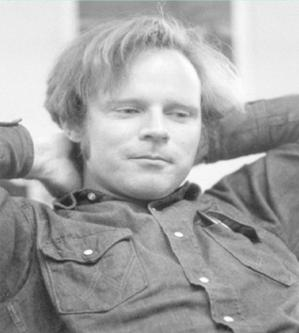
\includegraphics[width=.5\textwidth, height=.5\textheight,
            keepaspectratio]{algo/Floyd.jpg}

        \end{figure}
    \end{frame}

    \begin{frame}[t]
        \frametitle{Ý tưởng}
        \section{Ý tưởng}

    \end{frame}

    \begin{frame}[t]
        \frametitle{Cài đặt}
        \section{Cài đặt}
        while (a not sorted):
            generate a permutation from a.
    \end{frame}

    \begin{frame}[t]
        \section{Đánh giá}
        \frametitle{Đánh giá}
        \framesubtitle{Độ phức tạp thời gian}
        \begin{itemize}
            \item Độ phức tạp trong trường hợp tốt nhất: $\mathcal{O}(n^3)$
            \item Độ phức tạp trong trường hợp tệ nhất: $\mathcal{O}(n^3)$
            \item Độ phức tạp trung bình: $\mathcal{O}(n^3)$
        \end{itemize}
        \textbf{Nhận xét:} Thuật toán Floyd-Warshall có độ phức tạp khá \textbf{tệ} nhưng độ phức tạp mỗi truy vấn đường đi ngắn nhất sẽ là $\mathcal{O}(1)$.
    \end{frame}

    \begin{frame}[t]
        \frametitle{Đánh giá (cont.)}
        \framesubtitle{Độ phức tạp không gian}
        \begin{itemize}
            \item Độ phức tạp trong trường hợp tốt nhất: $\mathcal{O}(n^2)$
            \item Độ phức tạp trong trường hợp tệ nhất: $\mathcal{O}(n^2)$
            \item Độ phức tạp trung bình: $\mathcal{O}(n^2)$
        \end{itemize}
    \end{frame}

    \begin{frame}
        \frametitle{Tổng kết}
        \begin{itemize}
            \item Stupid Sort's poorly performance made it become an impractical sorting algorithm.
            \item May be used in some source code, but for \textbf{comparison} (w. other sorting algorithms) or \textbf{educational purpose} (e.g example for a poor-performance algorithm) only.
        \end{itemize}
    \end{frame}

    \begin{frame}
        \Large \centering
        The End!
    \end{frame}

    \begin{frame}[t]
        \frametitle{Tài liệu tham khảo}
        \section{Tài liệu tham khảo}
        \bibliographystyle{apalike}
        \begin{thebibliography}{10}
            \bibitem{names} Hello, world
        \end{thebibliography}
    \end{frame}


\end{document}